\documentclass{article}
\usepackage[utf8]{inputenc}
\usepackage{graphicx}
\usepackage{cleveref}
\usepackage{enumitem}

\title{First IDP Report}
\author{Group M213 ; Team 213 ; Robot 213}
\date{November 2022}

% To be confirmed that it requires the setspace package, try with and without.
\usepackage{setspace}

% Let top 85% of a page contain a figure
\renewcommand{\topfraction}{0.85}

% Default amount of minimum text on page (Set to 10%)
\renewcommand{\textfraction}{0.1}

% Only place figures by themselves if they take up more than 75% of the page
\renewcommand{\floatpagefraction}{0.75}

%zet de bladspiegel :
\setlength\paperwidth{20.999cm}\setlength\paperheight{29.699cm}\setlength\voffset{-1in}\setlength\hoffset{-1in}\setlength\topmargin{1.499cm}\setlength\headheight{12pt}\setlength\headsep{0cm}\setlength\footskip{1.131cm}\setlength\textheight{25cm}\setlength\oddsidemargin{2.499cm}\setlength\textwidth{16.5cm}

\begin{document}

\maketitle

% TODO: Please fill in your details in the table below

\begin{table}[]
    \centering
    \begin{tabular}{|c|c|c|c|}
        \hline
        Name &  CRsid & College & Lab Group \\
        \hline
        Matthew Hendricks & mah237 & Pembroke & 35 \\
        Louis Pender & lwp256 & & \\
        Hor Ye Heng & yhh35 & & \\
        Wen Yian & yw543 & & \\
        Yiheng Liu & yl827 & Lucy Cavendish & 13 \\
        Yuge & & & \\
        \hline
    \end{tabular}
    \caption{Coversheet information}
    \label{tab:Coversheet}
\end{table}


\newpage

\section{Introduction}
\quad The aim of this project is to design and build a robot that can navigate along a line track and collect and classify blocks of different densities. The competitions are marked using the following criteria:

\begin{itemize}
    \item Robot first traverses to other side of table (no part of robot on ramp or in tunnel) +10
    \item Robot traverses both ramp and tunnel +10
    \item Block delivered to correct area (entirely within lines) +10
    \item Block transported to delivery side of table +10
    \item Correct LED displayed to identify block +10
    \item Robot finally returns to a start/end box and stops such that the robot is entirely within the lines of the box. The robot must have made a sporting attempt to identify and collect blocks +20 
    \item 1st Competition only manual demonstration of block identification (block may be brought up to stationary robot by hand to demonstrate correct detection reliably) +10
\end{itemize}

\quad The arena layout can be seen in Figure \ref{fig:arena}. The robot must be able to traverse the ramp and tunnel, detect and deliver the blocks to the correct area. By traversing the ramp first before picking up the block, the robot can just push the block on the floor without lifting it which is far easier.

\quad To meet these criteria in the small timeline given our group was organised into mechanical, electrical and software teams. We also used a variety of tools to help us with our project management, design and collaberation.

\section{Project Management}
\quad L.W. Pender was selected as the leader of the group. We created a Trello project which has functionalities like a Gantt chart and Kanban boards as our project management systems. We made a rough timeline of the large milestones of the project such as having a fully assembled robot, having the sensors all attached onto the robot and funcitoning, having a working robot and testing, and placed these onto the Trello project. We then made smaller short-term goals for each team to achieve.
    
\section{Mechanical}
\quad The mechanical team consists of Pender, L.W. (lwp26) and Hendricks, M.A. (mah237). Our short term plan for the mechanical team was to get a good CAD model and a cardboard model out for the robot by the 14th of November. We started off by making some design decisions.

\subsection{Drive System}
\quad \quad We initially considered a few drive systems for the robot, namely a 3-wheeled differential drive system, a 4-wheeled tank drive system, making our own Mecanum wheels and a simple 2-wheeled system. 

\quad We ruled out the Mecanum wheels idea due to the sheer difficulty of manufacturing such a wheel without much added benefit to the project since the main priority for our team would be rapid production so that testing can begin sooner rather than later. The 3-wheeled differential drive was also ruled out due to not having 3 same-sized wheels. This is because we don't want the base of the chassis to be inclined in case we would have markers (such as QR codes) used by the software team for navigation and other purposes. The inclination would probably lead to larger errors in navigation. We ruled out the 4-wheeled tank drive system, as we were worried about slipping occuring in one of the sets of wheels if the ratios of the speeds were not accurate. This is especially important to us since we're thinking about using a light sensor as a rotary encoder to have an accurate measure of the distance travelled by the robot. A table summarising our comparisons can be seen in \Cref{tab:drive_comp}.

\quad Therefore, the best option we settled on was the simple 2-wheeled system, since it would be the simplest to manufacture. We plan to use the larger wheels so that our rotary encoder would be more accurate. The wheels will be connected to the higher torque lower RPM motor via the given motor adaptors. The higher torque will help in the robot going up the ramp. The motors will be attached to the robot by a metal bracket and bolting it onto the threads on the aluminium plate on the motor. We also will place a ball castor at the other end of the chassis to ensure the robot remains stable as it ascends the ramp.

\begin{table}[]
    \centering
    \begin{tabular}{|c|p{5cm}|p{5cm}|}
        \hline
        Idea & Advantages & Disadvantages \\
        \hline
        2-wheeled + Castor wheel & Fast to manufacture quickly& Might be harder to turn \\
        3-wheeled differential-drive & Easy to manufacture quickly & Might slip since wheels are not of same size \\
        4-wheeled tank drive system & Very reliable & More motors required and hard to sync the motor's rpm ratio due to different sized wheels \\
        \hline
    \end{tabular}
    \caption{Drive System Comparison}
    \label{tab:drive_comp}
\end{table}

\subsection{Chassis}
\quad After looking at the sizes of the various components (such as the Arduino and the battery pack) that we needed to fit onto the chassis we make a rough guess of a dimension of the base of the chassis to be $250mm \times 140mm$.

The chassis design for the prototype has been designed to be very modular, we have multiple holes for the components fitting locations so that we can swap the positions of the sensors and other components easily to redistribute the mass in the robot. We have laser cutted out parts of the chassis and are currently assembling the robot.

\subsection{Gripping Mechanism}
\quad We had 3 main ideas on how to capture the block. 

\quad The first was a simple pushing idea where we had a slight protrusion at the edges of the robot to ensure it doesn't get pushed off the robot. However this not only limits our route to be leaving the collection arena from the tunnel, it also is not reliable during turning.

\quad The second idea was to have a rack and pinion powering a moving stick to move closer to another stationary stick to grab the block. The problem with this was that the rack and pinion mechanism is less reliable and the block will be gripped to one side of the mechanism and the mass distribution will be shifted.

\quad The idea we settled on was to use a scissor like gripping mechanism as shown in \Cref{fig:grip_mech}. This might have slightly more parts but it is more reliable than the rack and pinion and the center of mass is not affected.

\subsection{Cardboard Model and CAD}
\quad We have made a cardboard model prototype for testing purposes as can be seen in \Cref{fig:cardboard_model}. This was laser cut out of cardboard and assembled using hot glue. The cardboard cut outs were designed first in a Solidworks model of the robot as can be seen in \Cref{fig:isometric}.

\section{Electrical}
\quad The electrical teams consists Hor Ye Heng (yhh35) and Yiheng Liu (yl827). We have finished designing what sensors to use for different functions and now working with the software team to test all the sensors.
\subsection{Overall Design}
\quad The tasks we are attempting to achieve are:
\begin{enumerate}
    \item Line sensing
    \begin{description}[leftmargin=-0.2in]
        \item[] For line sensing, we are using three line sensor OPB704 attached on the bottom of the vehicle to detect the lines. It returns different voltage depend on the reflection so able to detect while line and black surface.
    \end{description}
    \item Block detecting
    \begin{description}[leftmargin=-0.2in]
        \item[] For block detecting, two plans are going on together to compare which is better, one is to use ultrasonic and decide how much it passes through the block, another would be using light dependent resistor but will largely depend on the environment lighting.
    \end{description}
    \item Channel Guiding
    \begin{description}[leftmargin=-0.2in]
        \item[] A distance sensor will be used in the channel to keep the distance with the wall of the channel constant.
    \end{description}
\end{enumerate}
\subsection{Testing}
\begin{enumerate}
    \item OPB704 Line Sensor
    \begin{description}[leftmargin=-0.2in]
        \item[] Line sensor is already set up using correct resistors. When at a appropriate distance from the table surface, it returns about 1000 to the analog input of the Arduino when color is red, and 0-10 for white lines.
    \end{description}
    \item Ultrasonic Sensor
    \begin{description}[leftmargin=-0.2in]
        \item[] Our original plan is to use ultrasonic sensor to detect different density foams, considering the dense one would be likely to absorb ultrasonic wave and the wave may pass the other. By testing, we found it's likely that wave would pass both so we're still adjusting to see if it would work, otherwise we'll change to the light sensing route. 
    \end{description}
    \item Distance Sensor
    \begin{description}[leftmargin=-0.2in]
        \item[] Distance sensor is tested and work fine for distance above 10cm. Above 10cm, the analog input from the distance sensor is proportional to the distance form obstacle and is set up for software team to test.
    \end{description}
\end{enumerate}
\section{Software}
\subsection{Arduino Firmware}
% Yuge and Steve please fill in your work here %
\subsection{OpenCV}
\subsubsection{Overall Plan}
This branch of the project is currently in the nightly stage, i.e. we are only exploring the feasibility of using computer vision, powered by the OpenCV library, to carry out path planning around the arena and therefore offloading the navigation of the robot entirely to a PC.

Should this be successful, the overall operation would involve streaming the live video feed from the overhead webcams into a Python script, which would carry out the following processing steps:
\begin{enumerate}
    \item World Mapping 
    \begin{description}[leftmargin=-0.2in]
        \item The script would detect all the features within the field of view such as the white path lines, the red and green squares, and the lime colored obstacle. A map of the arena would be constructed from the location information of these features, and cached into memory.
    \end{description}
    \item Navigate to Payload
    \begin{description}[leftmargin=-0.2in]
        \item[] In this state, the script waits for the presence of the target payload (the foam blocks). Once a foam block is detected, a pathfinding algorithm would be run to establish a path from the current robot position to the position of the foam blocks. Commands will then be sent to the robot to move according to the aforementioned path.
    \end{description}
    \item Navigate to Goal Area
    \begin{description}[leftmargin=-0.2in]
        \item[] In a similar manner, once the foam block has been picked up and it's category determined, the path planning algorithm infers a path from the current robot position to the goal area. Commands will then be sent to the robot to carry out the required movements.
    \end{description}
\end{enumerate}

We plan to use UDP packets to stream commands to the Arduino on the robot, which would be configured to be an access point so that we have a dedicated data pipe that will not be affected by inconsistencies of the network infrastructure in the department. However, should the handling of the UDP packets become too much of a challenge, we could fall back to sending HTTP requests to command the Arduino - an approach that has been well documented by others within the maker community.

\subsubsection{Potential Issues and Ways to Mitigate Them}
\begin{enumerate}
    \item Latency
    \begin{description}[leftmargin=-0.2in]
        \item[] We noticed that OpenCV buffers frames as they come in over the MJPEG stream, and therefore, with our current naive implementation, the speed at which the processing loop runs determines how much the current frame being processed lags behind real time.
        \item[] This should be an easy fix, a thread could be spawned to clear out the frame buffer such that the current frame being read by the processing loop is never stale.
    \end{description}
    \item Network Dropout
    \begin{description}[leftmargin=-0.2in]
        \item[] We were informed multiple times by various parties that network stability was a huge issue for teams in the past.
        \item[] In the event that issues with 802.11b/g/n network congestion become significant, the ESP32 on board the Arduino also has native support for Bluetooth Low Energy (BLE), which implements frequency hopping specifically to combat congestion, so we would switch over to using BLE for communication between the PC and the Arduino.
    \end{description}
\end{enumerate}


\section{Appendix}
% Please put all of your image documents in the asset folder and place all of your figures here. TQ
\begin{figure}[!h]
    \centering
    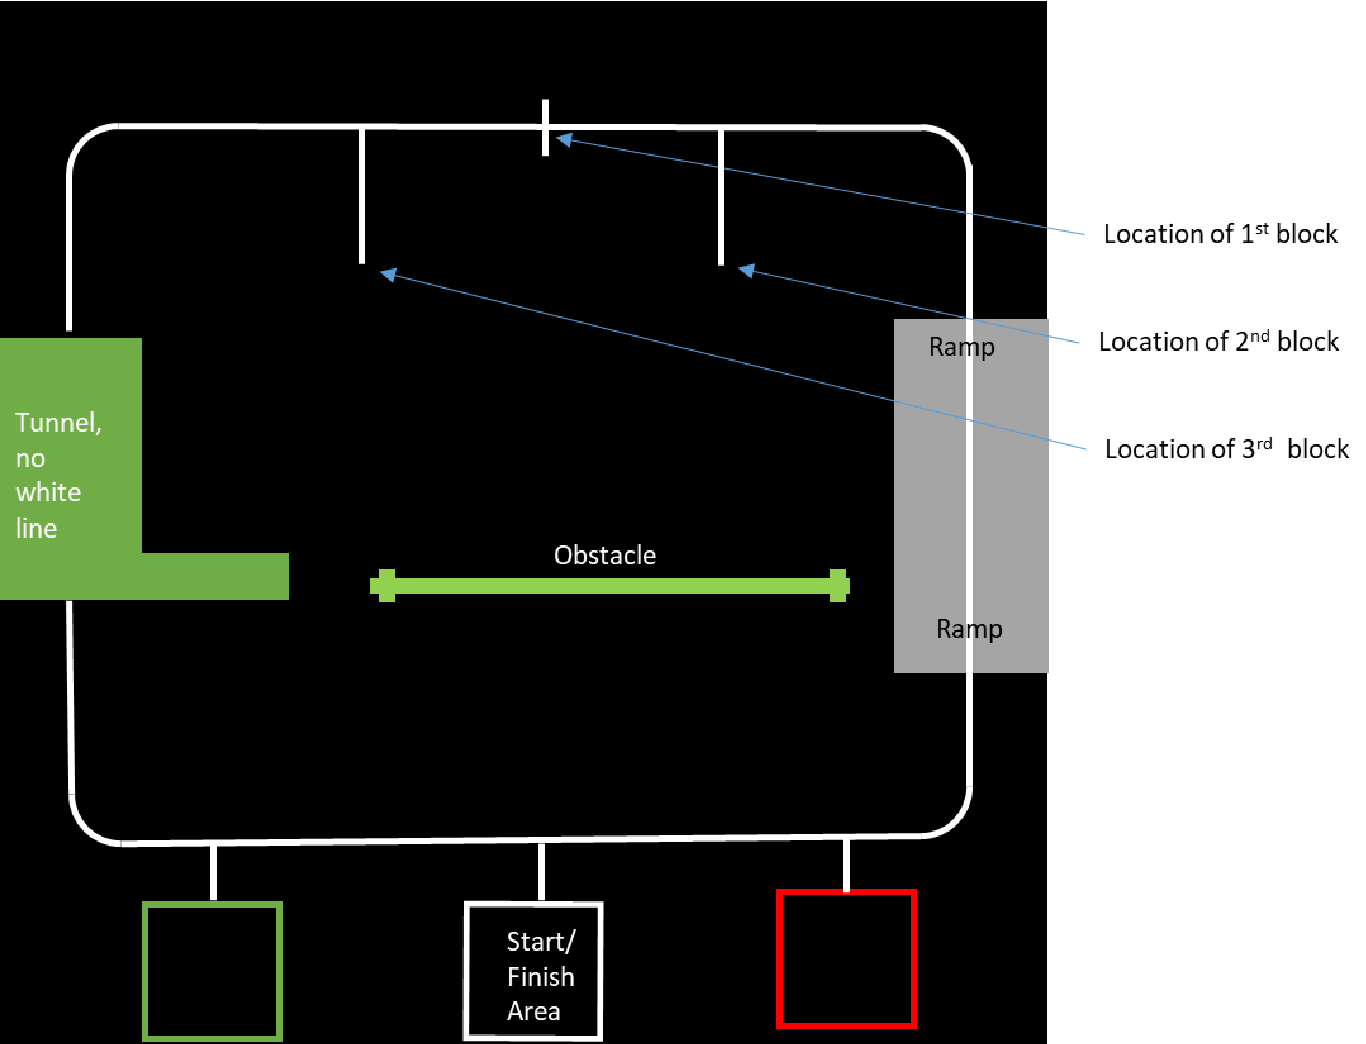
\includegraphics[width=0.8\textwidth]{assets/arena.png}
    \caption{Arena picture}
    \label{fig:arena}
\end{figure}

\begin{figure}[!h]
    \centering
    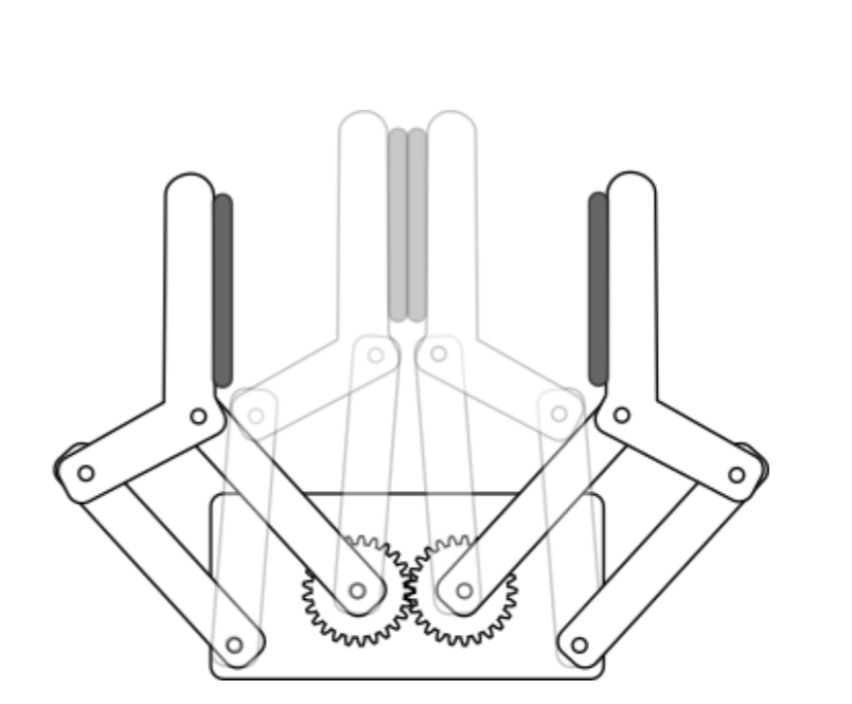
\includegraphics[width=0.8\textwidth]{assets/Gripper_Mechanism.jpg}
    \caption{Scissor-like Gripper Mechanism}
    \label{fig:grip_mech}
\end{figure}

\begin{figure}[!h]
    \centering
    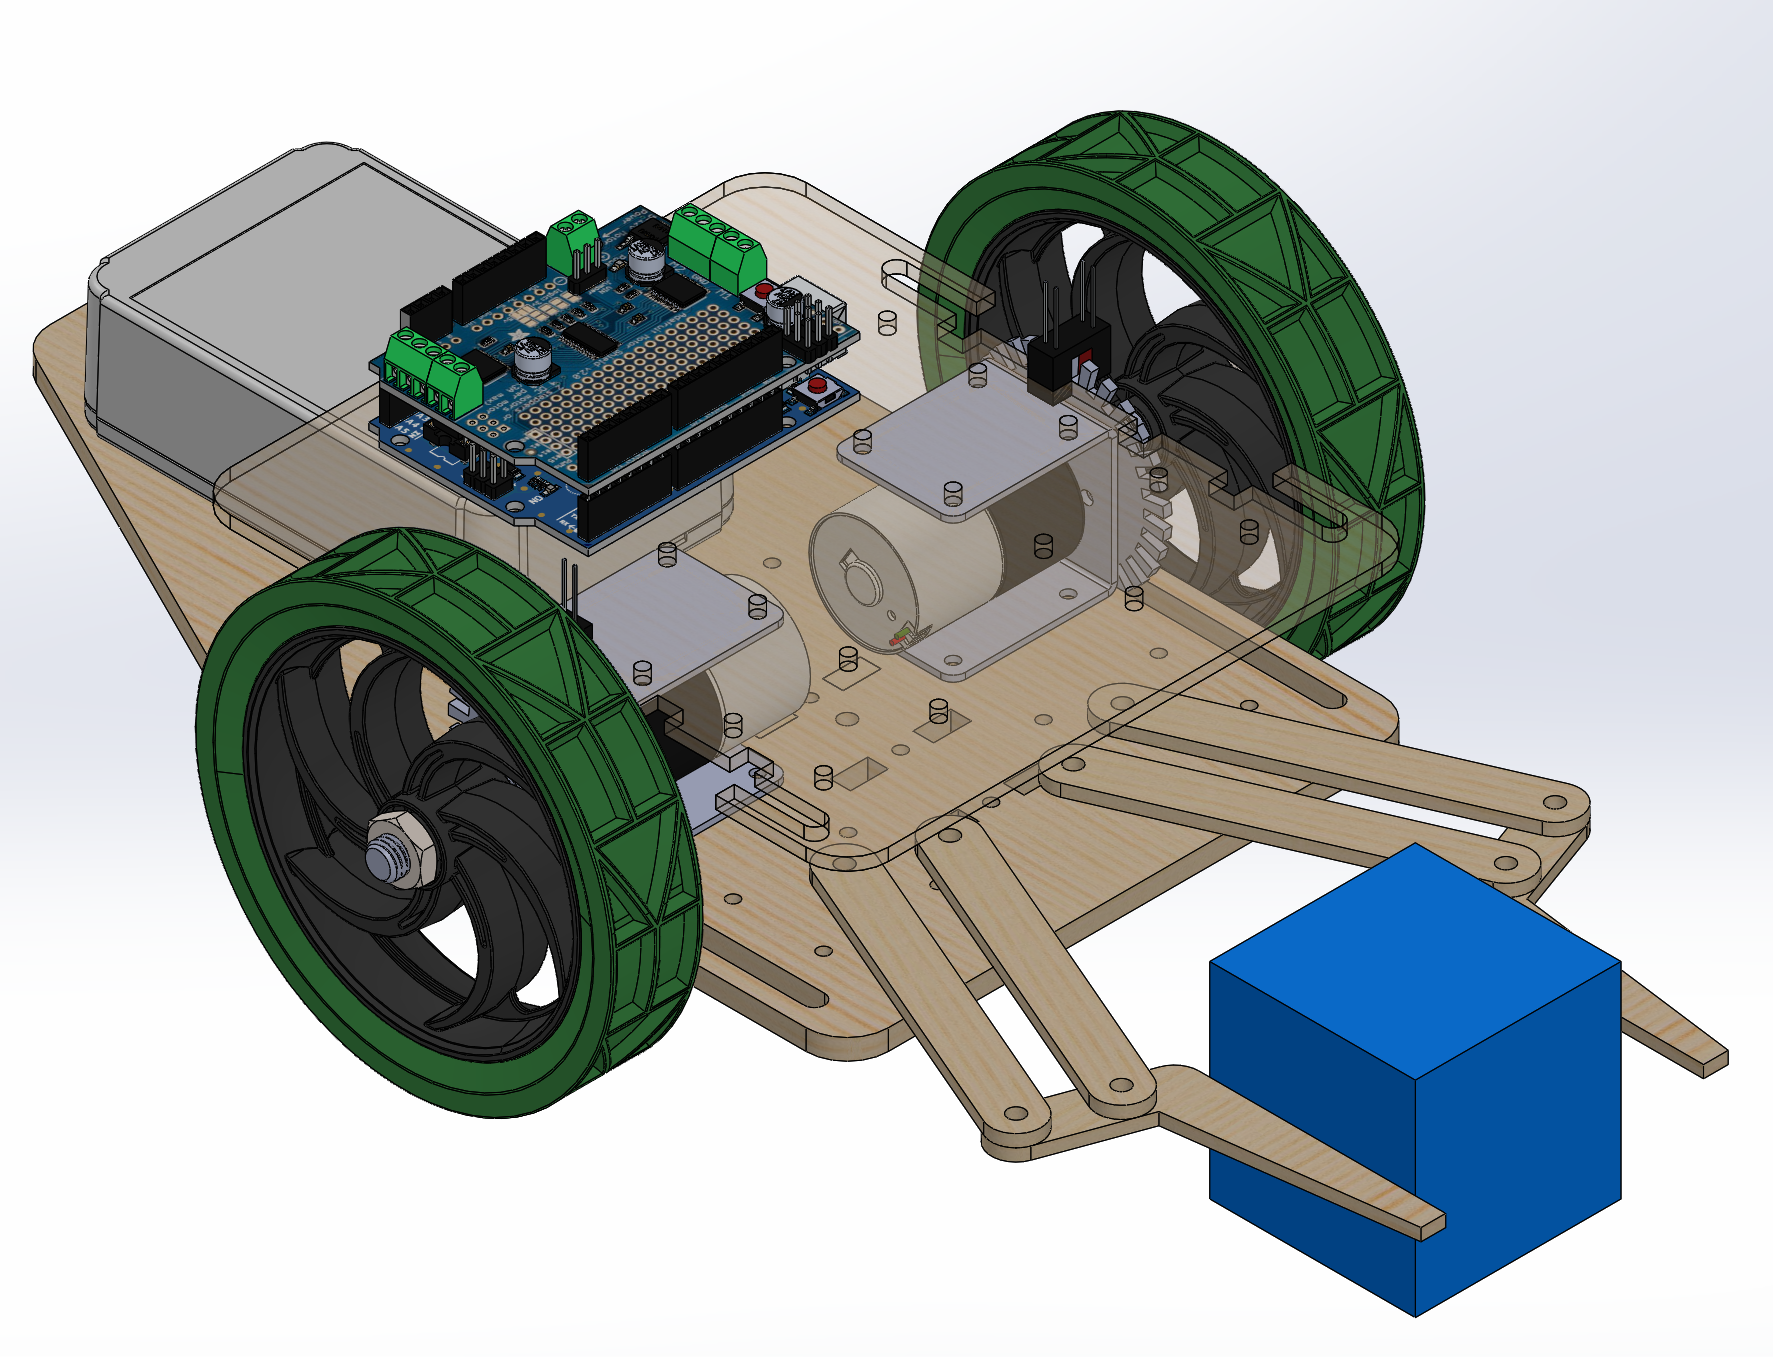
\includegraphics[width=0.8\textwidth]{assets/isometric.png}
    \caption{Current Isometric Solidworks Model}
    \label{fig:isometric}
\end{figure}

\begin{figure}[!h]
    \centering
    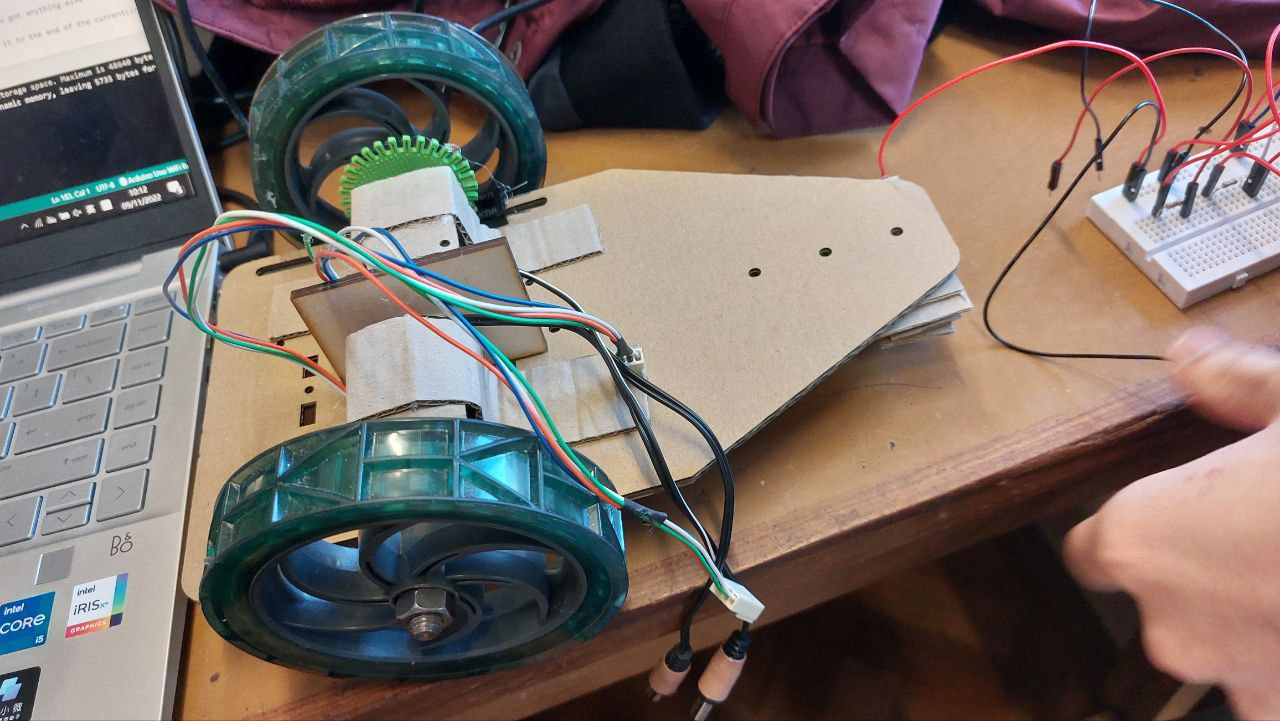
\includegraphics[width=0.8\textwidth]{assets/Cardboard_model.jpg}
    \caption{Cardboard Model}
    \label{fig:cardboard_model}
\end{figure}

\begin{figure}[!h]
    \centering
    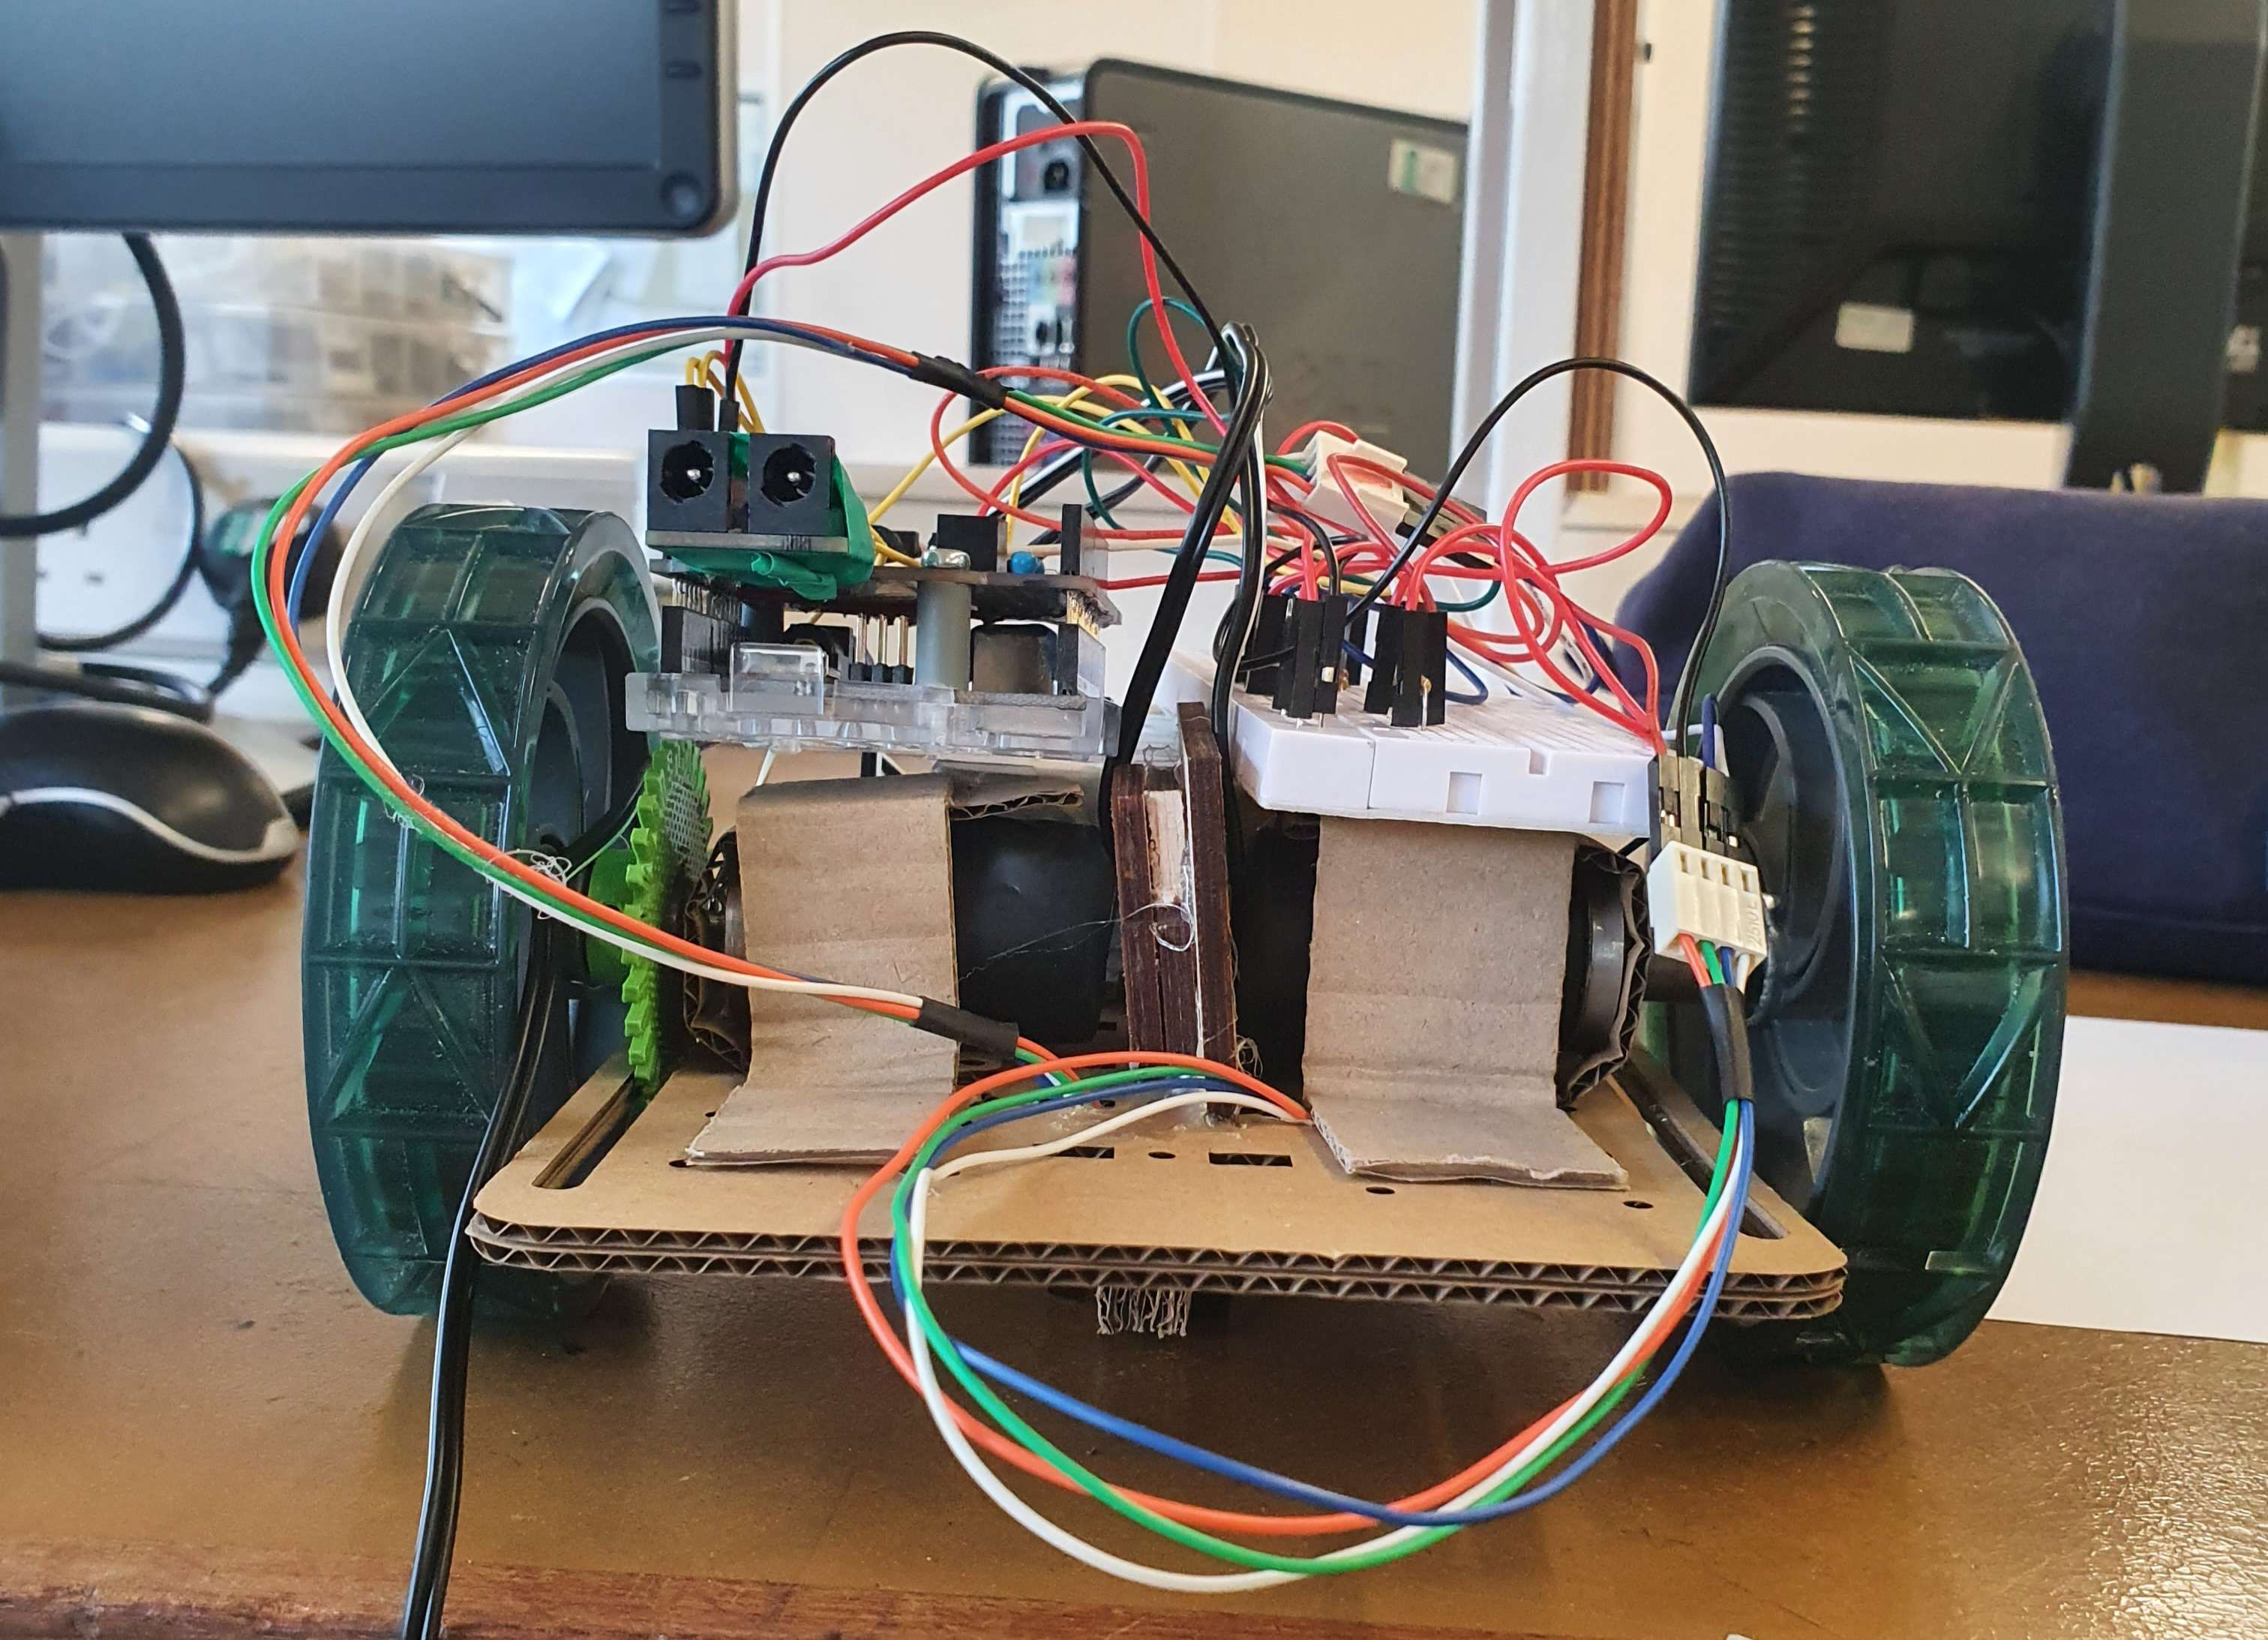
\includegraphics[width=0.8\textwidth]{assets/assembled_prototype.jpg}
    \caption{Assembled Prototype}
    \label{fig:assembled_prototype}
\end{figure}


\end{document}
